\section{ttbb}
\label{sec:ttbb}

\subsection{Samples}
Four MC generators are compared in this study, where the inclusive $\mathrm{t\bar{t}}$ PP8 sample was previously used as the nominal background estimate in the ttH analysis. It is generated with the \textsc{POWHEG-BOX v2} NLO event generator~\cite{Nason:2004rx,Frixione:2007vw,Alioli:2010xd,Campbell:2014kua} with NNPDF3.0 NLO PDF set, matched to Pythia8 and is referred to as PP8 $\mathrm{t\bar{t}}$, where the additional bb-pair is described by the parton shower. The $h_{damp}$ parameter was set to 1.5 times the top quark mass~\cite{ATL-PHYS-PUB-2016-020}, which is assumed to be 172.5 GeV. The parton shower and the hadronisation were modelled by Pythia 8.210 with the A14 set of tuned parameters. The renormalisation and factorisation scales were set to the transverse mass of the top quark.
The intrinsic uncertainty of the nominal PP8 $\mathrm{t\bar{t}}$ sample is expressed by the simultaneous variation of the renormalisation and factorisation scales together with the PDF tune parameter. The RadiationUp variation has the renormalisation and factorisation scales decreased by a factor of two, the Var3c upward variation of the A14 parameter set and the $h_{damp}$ parameter doubled. The RadiationDown variation has the renormalisation and factorisation scales increased by a factor of two, the Var3c downward variation and the nominal value of $h_{damp}$.
Additionally, the up and down radiation uncertainty is calculated following the CMS approach , under which the renormalisation scale, factorisation scale and PDF tune variations are each taken individually and their difference to the nominal is summed in quadrature.

The PP8 tt+bb sample also uses the POWHEG generator where $t\bar{t}b\bar{b}$ matrix elements are calculated at NLO with massive b-quarks, using the four-flavour NLO NNPDF3.0 PDF set~\cite{Jezo:2018yaf}. The parton shower and hadronisation is modelled by Pythia 8.240.

For the PP8 samples the bottom and charm quark decays are described by EVTGEN v1.2~\cite{LANGE2001152} and the top quark spin correlations follow reference~\cite{Frixione:2007zp}.

The \textsc{Sherpa} tt+bb sample describes NLO tt+bb including parton showering and hadronisation by \textsc{Sherpa}-\textsc{Openloops}~\cite{Cascioli:2013era,Gleisberg:2008ta,Cascioli:2011va}. The sample was produced with Sherpa version 2.1.1 and the CT10 four-flavour scheme PDF set~\cite{Guzzi:2011sv,Gao:2013xoa} The renormalisation scale is set to the CMMPS value as in ref~\cite{Cascioli:2013era}, the factorisation and resummation scales equal $\mathrm{H_T/2}$.

Both the PP8 tt+bb and the \textsc{Sherpa} tt+bb samples describe the additional bb-pair with NLO precision in QCD, taking into account the b-quark mass

The \textsc{Sherpa} $\mathrm{t\bar{t}}$ sample uses \textsc{Sherpa} version 2.2.1~\cite{Gleisberg:2008ta} with the ME+PS@NLO (multi-leg) setup using the MEPS@NLO prescription~\cite{Hoeche:2012yf}, interfaced with \textsc{Openloops}. It provides NLO accuracy for up to one additional parton and LO accuracy for up to four additional partons. The NNPDF3.0 NNLO PDF set is used with a five-flavour scheme and both renormalisation and factorisation scales are set to $\sqrt{0.5\times(m_{T,t}^2+m_{T,\bar{t}}^2)}$. 
A summary of all samples used is given in Table~\ref{tab:ttbbsamples}.

\begin{table}
\begin{center}
\caption{\label{tab:ttbbsamples}
The configurations used for the event generation of ttbb processes.}
\vspace{0.25cm}
{\small
\setlength\tabcolsep{1.5pt}
\begin{tabular}{llllll}
\hline\hline
Process & Generator & ME order & Parton shower & PDF & Tune  \\
%& (alternative) & (alternative) & & \\
\hline
$\ttbar$  & \textsc{PowHeg v2} & \textsc{NLO} & \textsc{Pythia 8} &  5FS NNPDF3.0 NNLO & \textsc{A14}  \\
$\ttbar+b\bar{b}$  & \textsc{PowHeg v2} & \textsc{NLO} & \textsc{Pythia 8} &  4FS NNPDF3.0 NNLO & \textsc{A14}  \\
$\ttbar+b\bar{b}$  & \textsc{Sherpa 2.1.1} & \textsc{NLO} & \textsc{Sherpa} &  4FS NNPDF3.0 NNLO & \textsc{Sherpa} default  \\
$\ttbar$  & \textsc{Sherpa 2.2.1} & tt+0,1p\@NLO+3p@LO & \textsc{Sherpa} &  5FS NNPDF3.0 NNLO & \textsc{Sherpa} default  \\
\hline\hline
\end{tabular}
}
\end{center}
\end{table}

\subsection{Fiducial Volume}
Object and event selection is defined at particle-level that closely matches the detector-level described in reference~\cite{HIGG-2017-03}. Jets are reconstructed from stable particles with a mean lifetime of $\tau > 3\times 10^{-11}$~s, using the anti-$k_t$ algorithm with a radius parameter of $R=0.4$, and are required to have $\mathrm{p_{T}>25 GeV}$ and $|\eta|< 2.5$. Jets are matched to b-hadrons with $\mathrm{p_{T}>5 GeV}$ by ghost matching~\cite{Cacciari:2008gn} and are referred to as b-jets. Electrons and muons, referred to as leptons, are required to satisfy $\mathrm{p_{T}>27 GeV}$. Selected leptons are required to be separated from selected jets by $\Delta R>0.4$. Events are selected with exactly one lepton and at least 4 jets, targeting the semi-leptonic $\mathrm{t\bar{t}}$ decay.
Two regions are considered, defined by 3 b-jets or $\geq$4 b-jets.

\subsection{Results}
The nominal PP8 $\mathrm{t\bar{t}}$ sample is compared to its radiation uncertainty variations and alternative generators, scaled to a common arbitrary integrated luminosity.
The first ratio plot shows the ratio of the different MC samples to PP8 $\mathrm{t\bar{t}}$, where the colour scheme is given in the legend.
Discrepancies between PP8 $\mathrm{t\bar{t}}$ and the alternative generators can be seen in the $\Delta R$ quantities, as in Figures~\ref{ttbb:avedR} and \ref{ttbb:mindR}, where at least in the 4b selection the difference to the alternative generators is larger than the uncertainty band given by the radiation variations.  
In the b-jet pair invariant mass variables $\mathrm{M_{bb}^{max P_T}}$ and $\mathrm{M_{bb}^{min \Delta R}}$ shown in Figures~\ref{ttbb:MbbmaxPT} and~\ref{ttbb:MbbminDR}, the largest difference is seen between the Sherpa $\mathrm{t\bar{t}}$ and all other samples.
Differences are also observed in the $\mathrm{H_T}$ distributions, particularly in the 3b selection. In $\mathrm{H_T}$ of all b-jets, as in Figures~\ref{ttbb:HTbjets}, one observes a difference between the 4 and 5 flavour schemes, while in $\mathrm{H_T}$ of all light jets, shown in Figure~\ref{ttbb:HTljets} a difference between PP8 $\mathrm{t\bar{t}}$ and the samples with b-jets in the ME can be seen. The jet multiplicity, as in Figure~\ref{ttbb:Njets}, has poor agreement among the generators for large jet multiplicities.
Lastly, differences among the samples are shown for the $\mathrm{\eta_{jet}}$ distribution, in Figure~\ref{ttbb:jeteta}.

The second ratio plot shows the relative uncertainty of the radiation variations, shown as the ratio of the uncertainty to the nominal for three cases. The PP8 $\mathrm{t\bar{t}}$ sample (black) and the PP8 tt+bb sample (blue), following the above description. It can be seen that the this type of uncertainties is larger for the tt+bb case than in the $\mathrm{t\bar{t}}$ calculation.
Also, the sum of individual variations following the CMS approach (red) on PP8 $\mathrm{t\bar{t}}$ leads to a smaller uncertainty with respect to the simultaneous variation.


\begin{figure}[!htb]
\centering
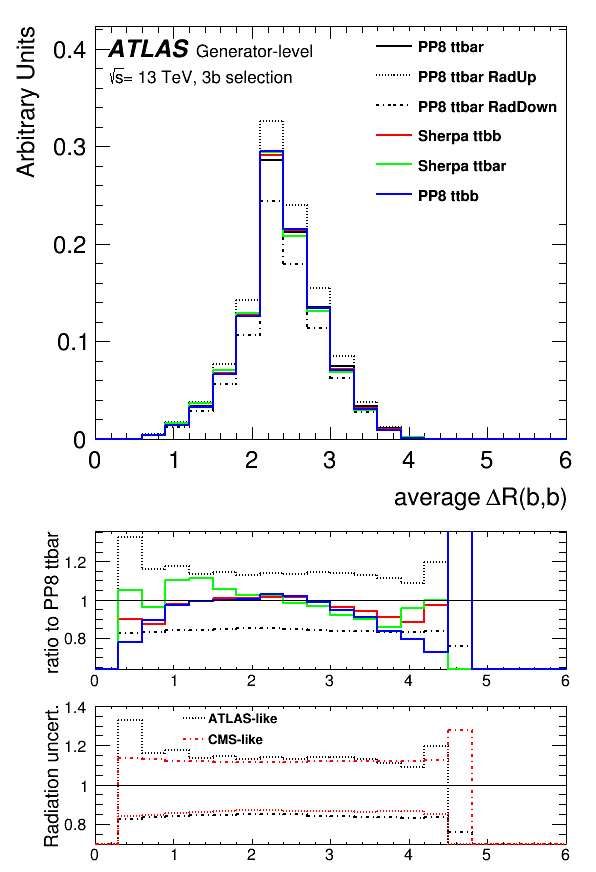
\includegraphics[width=0.38\textwidth]{Plots/ttbb/hisgenEvt_Dr_GenBJetsAverage_4j3t__div}
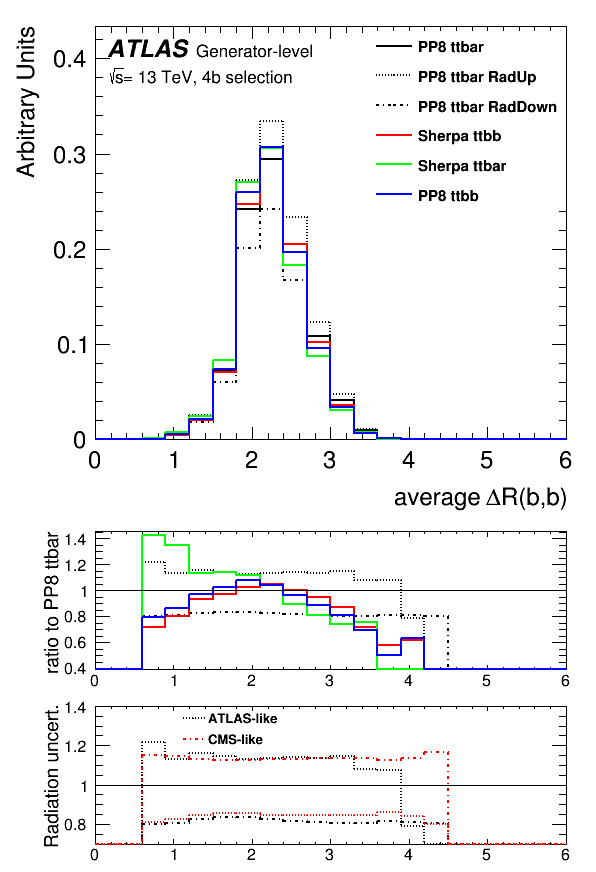
\includegraphics[width=0.38\textwidth]{Plots/ttbb/hisgenEvt_Dr_GenBJetsAverage_4j4t__div}
  \caption{Distribution of the average opening angle between two b-jets, for the 3b selection (left) and the 4b-jet selection (right). The first ratio plot shows the ratio of the different MC samples to PP8 $\mathrm{t\bar{t}}$, together with its radiation uncertainties. The second ratio plot shows the relative uncertainty of the radiation variations divided by the nominal, for PP8 $\mathrm{t\bar{t}}$ (black) PP8 tt+bb (blue), following the above description of simultaneous variations. The sum of individual variations following the CMS approach (red) is shown for PP8 $\mathrm{t\bar{t}}$.  \label{ttbb:avedR}}
\end{figure}

\begin{figure}[!htb]
\centering
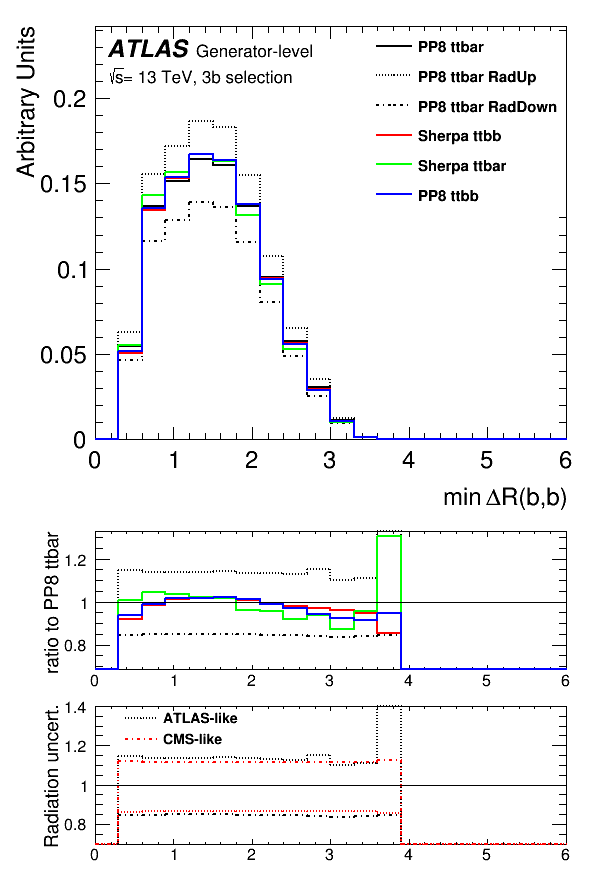
\includegraphics[width=0.38\textwidth]{Plots/ttbb/hisgenEvt_Dr_MinDeltaRGenBJets_4j3t__div}
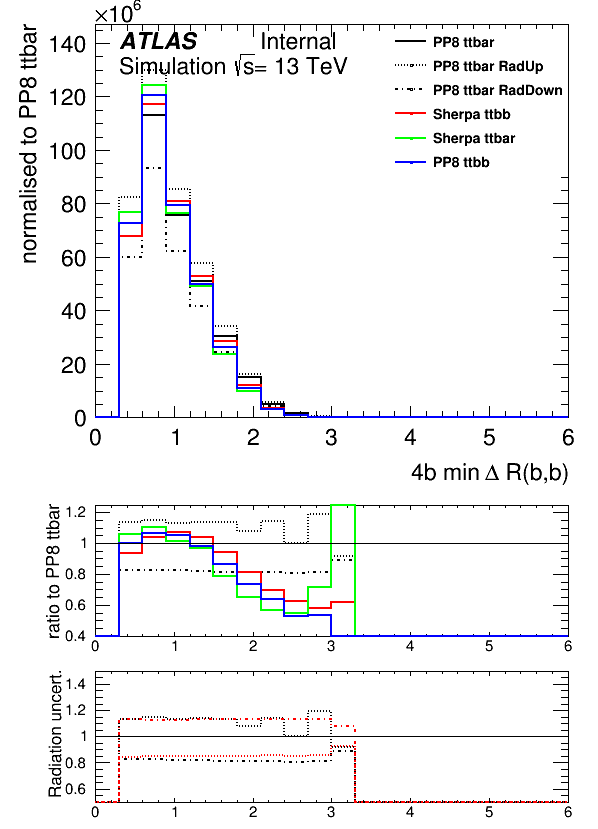
\includegraphics[width=0.38\textwidth]{Plots/ttbb/hisgenEvt_Dr_MinDeltaRGenBJets_4j4t__div}
  \caption{Distribution of the smallest opening angle between two b-jets, for the 3b selection (left) and the 4b-jet selection (right). The first ratio plot shows the ratio of the different MC samples to PP8 $\mathrm{t\bar{t}}$, together with its radiation uncertainties. The second ratio plot shows the relative uncertainty of the radiation variations divided by the nominal, for PP8 $\mathrm{t\bar{t}}$ (black) PP8 tt+bb (blue), following the above description of simultaneous variations. The sum of individual variations following the CMS approach (red) is shown for PP8 $\mathrm{t\bar{t}}$. \label{ttbb:mindR}}
\end{figure}

\begin{figure}[!htb]
\centering
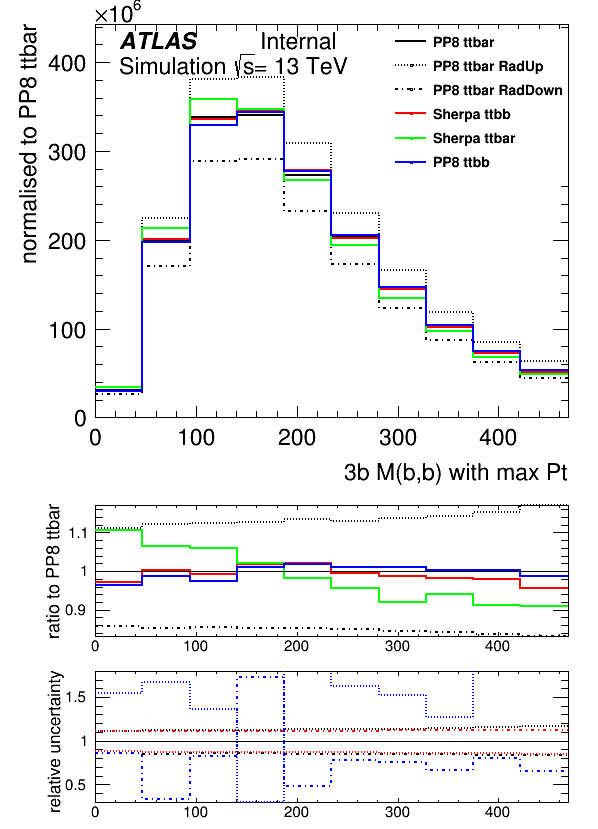
\includegraphics[width=0.38\textwidth]{Plots/ttbb/hisgenEvt_M_HardestGenBJets_4j3t__div}
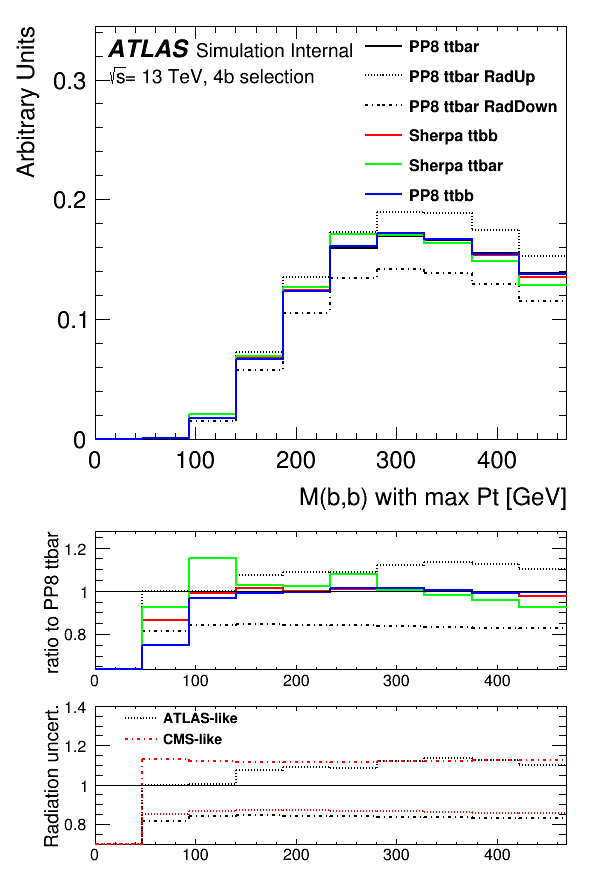
\includegraphics[width=0.38\textwidth]{Plots/ttbb/hisgenEvt_M_HardestGenBJets_4j4t__div}
  \caption{Distribution of the invariant mass in GeV of the two b-jets with the highest $\mathrm{P_T}$ sum, for the 3b selection (left) and the 4b-jet selection (right). The first ratio plot shows the ratio of the different MC samples to PP8 $\mathrm{t\bar{t}}$, together with its radiation uncertainties. The second ratio plot shows the relative uncertainty of the radiation variations divided by the nominal, for PP8 $\mathrm{t\bar{t}}$ (black) PP8 tt+bb (blue), following the above description of simultaneous variations. The sum of individual variations following the CMS approach (red) is shown for PP8 $\mathrm{t\bar{t}}$. \label{ttbb:MbbmaxPT}}
\end{figure}

\begin{figure}[!htb]
\centering
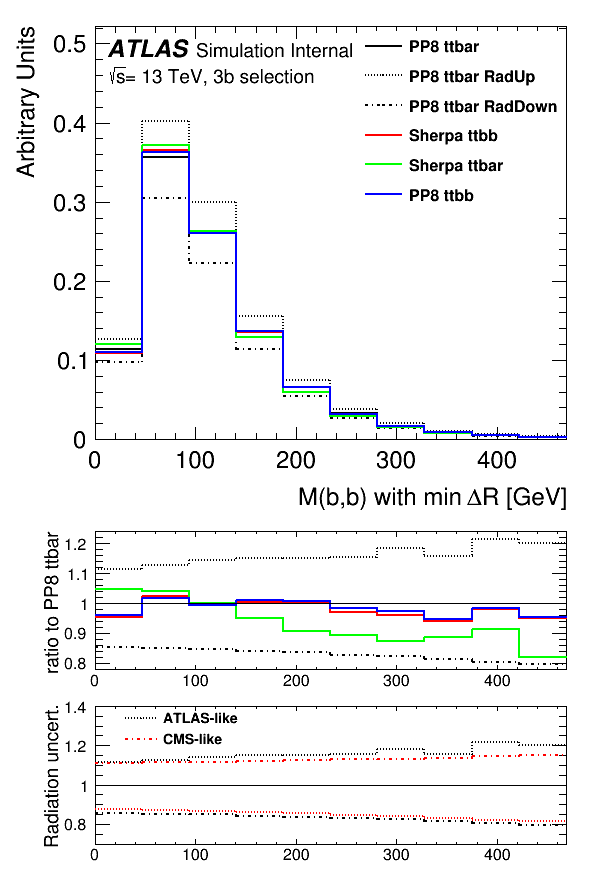
\includegraphics[width=0.38\textwidth]{Plots/ttbb/hisgenEvt_M_MinDeltaRGenBJets_4j3t__div}
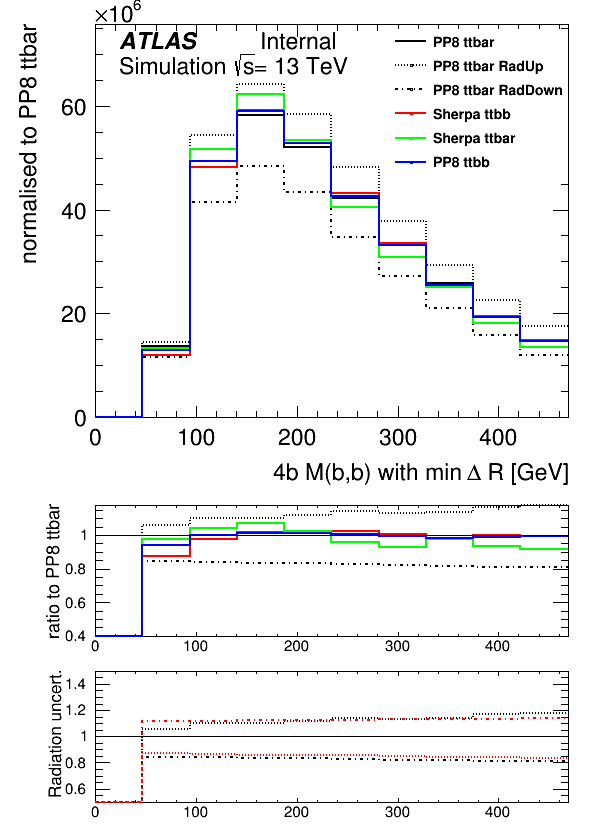
\includegraphics[width=0.38\textwidth]{Plots/ttbb/hisgenEvt_M_MinDeltaRGenBJets_4j4t__div}
  \caption{Distribution of the invariant mass in GeV of the two b-jets with the smallest opening angle, for the 3b selection (left) and the 4b-jet selection (right). The first ratio plot shows the ratio of the different MC samples to PP8 $\mathrm{t\bar{t}}$, together with its radiation uncertainties. The second ratio plot shows the relative uncertainty of the radiation variations divided by the nominal, for PP8 $\mathrm{t\bar{t}}$ (black) PP8 tt+bb (blue), following the above description of simultaneous variations. The sum of individual variations following the CMS approach (red) is shown for PP8 $\mathrm{t\bar{t}}$. \label{ttbb:MbbminDR}}
\end{figure}

\begin{figure}[!htb]
\centering
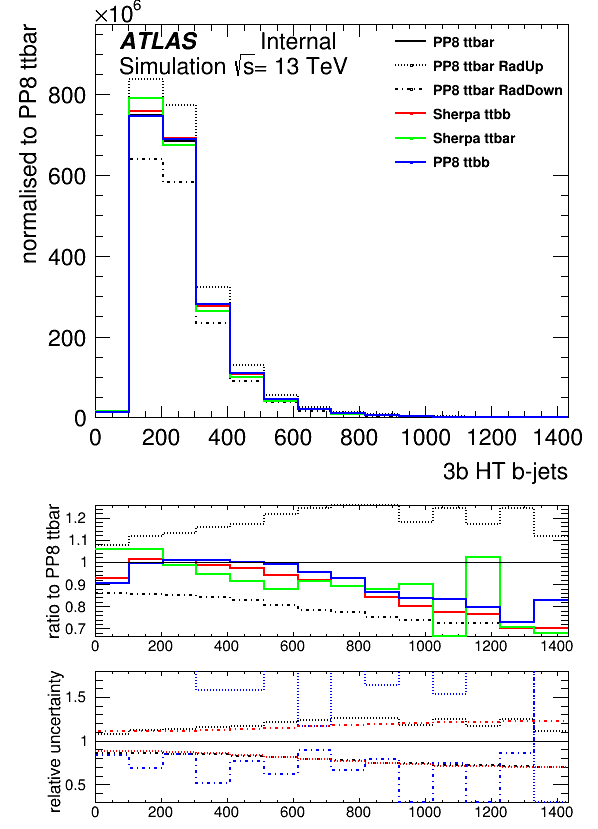
\includegraphics[width=0.38\textwidth]{Plots/ttbb/hisgenHTbjets_4j3t__div}
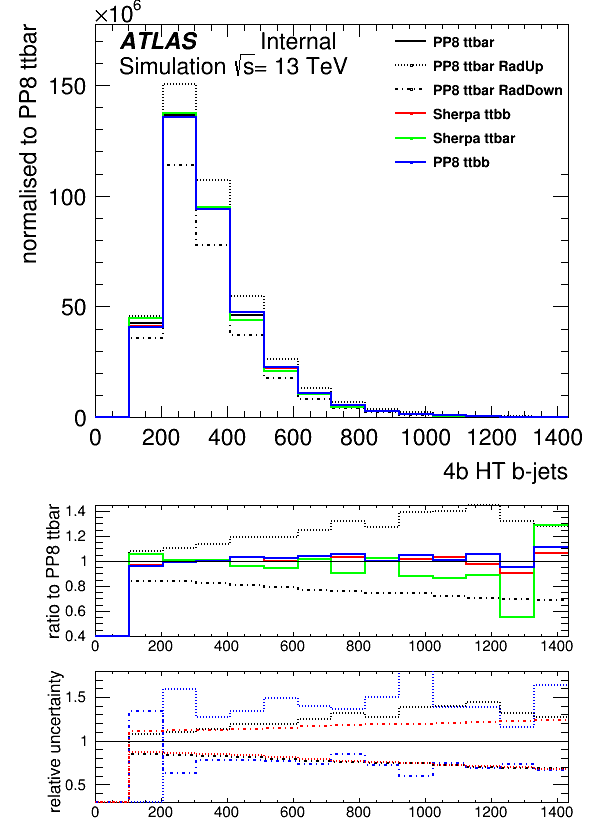
\includegraphics[width=0.38\textwidth]{Plots/ttbb/hisgenHTbjets_4j4t__div}
  \caption{Sum of b-jet transverse momenta in GeV, for the 3b selection (left) and the 4b-jet selection (right). The first ratio plot shows the ratio of the different MC samples to PP8 $\mathrm{t\bar{t}}$, together with its radiation uncertainties. The second ratio plot shows the relative uncertainty of the radiation variations divided by the nominal, for PP8 $\mathrm{t\bar{t}}$ (black) PP8 tt+bb (blue), following the above description of simultaneous variations. The sum of individual variations following the CMS approach (red) is shown for PP8 $\mathrm{t\bar{t}}$. \label{ttbb:HTbjets}}
\end{figure}

\begin{figure}[!htb]
\centering
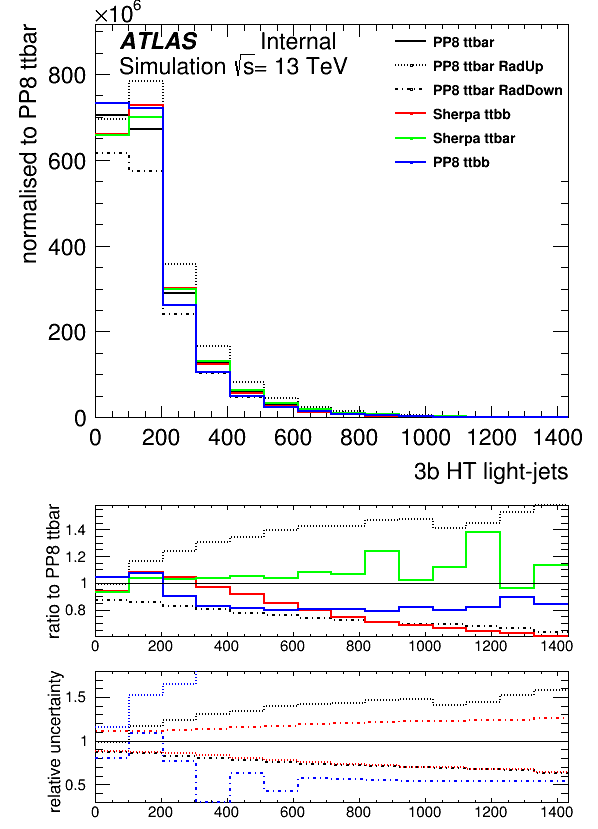
\includegraphics[width=0.38\textwidth]{Plots/ttbb/hisgenHTljets_4j3t__div}
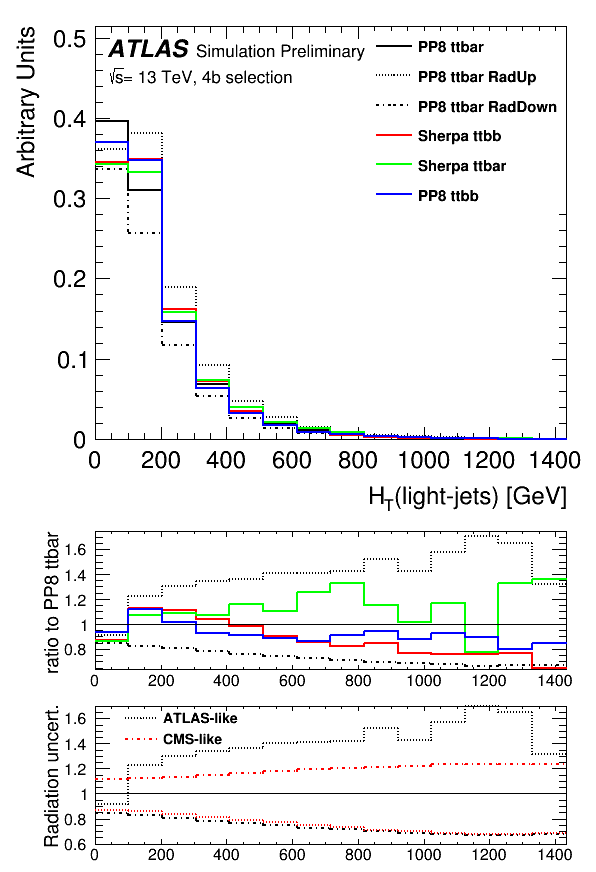
\includegraphics[width=0.38\textwidth]{Plots/ttbb/hisgenHTljets_4j4t__div}
  \caption{Sum of non-b-jet transverse momenta in GeV, for the 3b selection (left) and the 4b-jet selection (right). The first ratio plot shows the ratio of the different MC samples to PP8 $\mathrm{t\bar{t}}$, together with its radiation uncertainties. The second ratio plot shows the relative uncertainty of the radiation variations divided by the nominal, for PP8 $\mathrm{t\bar{t}}$ (black) PP8 tt+bb (blue), following the above description of simultaneous variations. The sum of individual variations following the CMS approach (red) is shown for PP8 $\mathrm{t\bar{t}}$. \label{ttbb:HTljets}}
\end{figure}

\begin{figure}[!htb]
\centering
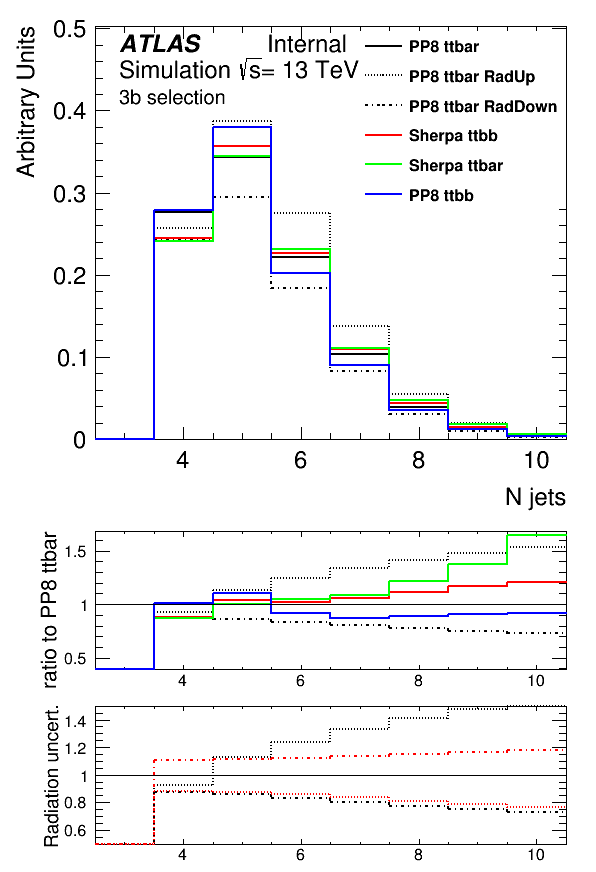
\includegraphics[width=0.38\textwidth]{Plots/ttbb/hisgenNjets_4j3t__div}
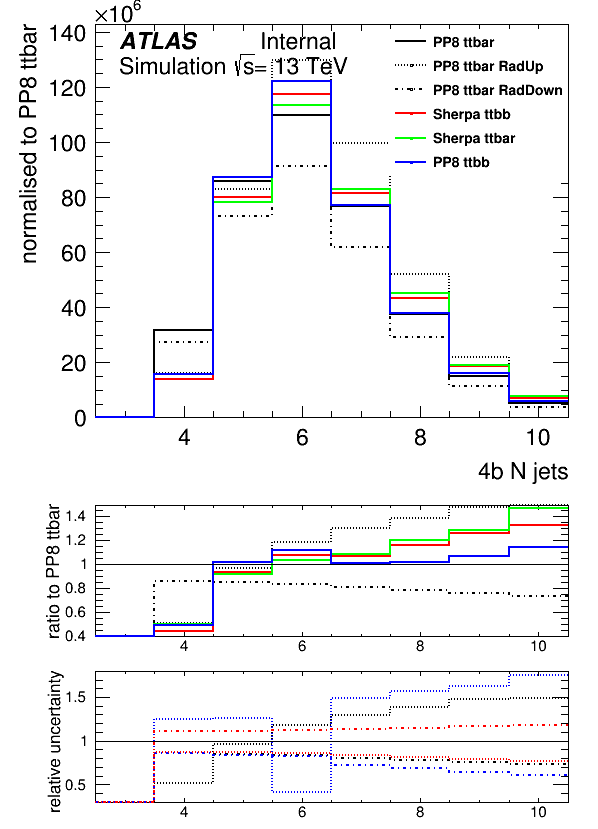
\includegraphics[width=0.38\textwidth]{Plots/ttbb/hisgenNjets_4j4t__div}
  \caption{Jet multiplicity, for the 3b selection (left) and the 4b-jet selection (right). The first ratio plot shows the ratio of the different MC samples to PP8 $\mathrm{t\bar{t}}$, together with its radiation uncertainties. The second ratio plot shows the relative uncertainty of the radiation variations divided by the nominal, for PP8 $\mathrm{t\bar{t}}$ (black) PP8 tt+bb (blue), following the above description of simultaneous variations. The sum of individual variations following the CMS approach (red) is shown for PP8 $\mathrm{t\bar{t}}$. \label{ttbb:Njets}}
\end{figure}

\begin{figure}[!htb]
\centering
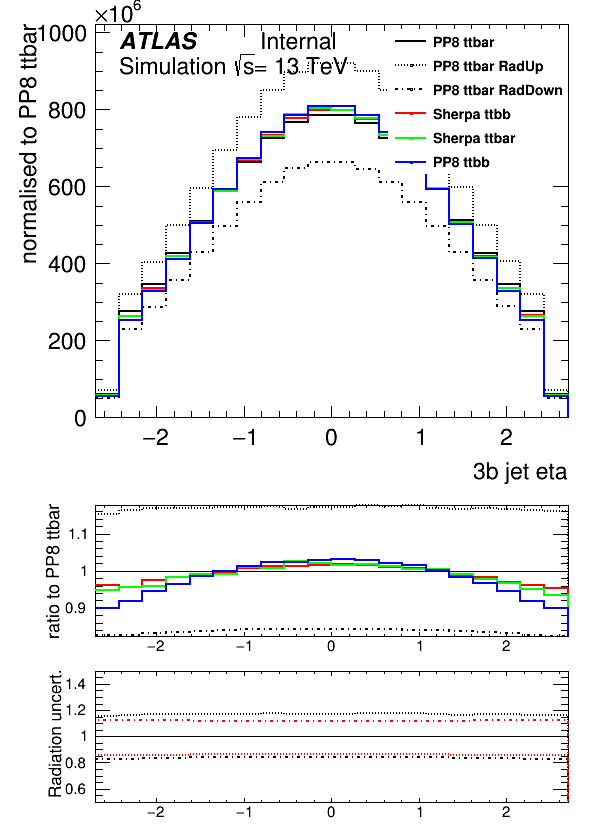
\includegraphics[width=0.38\textwidth]{Plots/ttbb/his3b_jeteta__div}
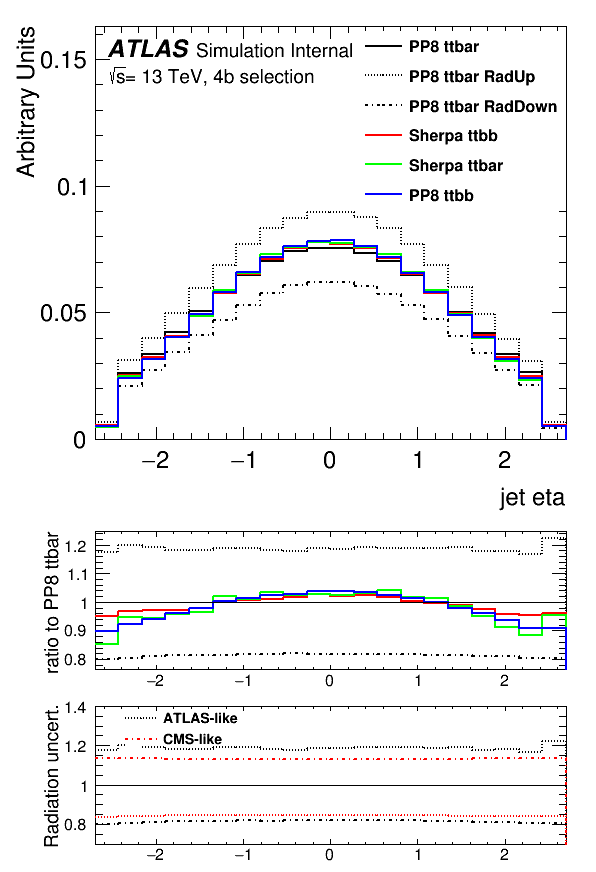
\includegraphics[width=0.38\textwidth]{Plots/ttbb/his4b_jeteta__div}
  \caption{Jet pseudorapidity, for the 3b selection (left) and the 4b-jet selection (right). The first ratio plot shows the ratio of the different MC samples to PP8 $\mathrm{t\bar{t}}$, together with its radiation uncertainties. The second ratio plot shows the relative uncertainty of the radiation variations divided by the nominal, for PP8 $\mathrm{t\bar{t}}$ (black) PP8 tt+bb (blue), following the above description of simultaneous variations. The sum of individual variations following the CMS approach (red) is shown for PP8 $\mathrm{t\bar{t}}$. \label{ttbb:jeteta}}
\end{figure}